\begin{exercise}
      {ID-18e18708d8d2556756e8bbe48ca99cc674e80029}
      {Gummibärchen}
  \ifproblem\problem\par
    % <PROBLEM>
    \xya{} und \xxb{} würfeln abwechselnd um Gummibärchen. \xya{} gewinnt bei den
    Augenzahlen 1, 2, 3 oder 4, \xxb{} gewinnt bei 5 oder 6. Der Gewinner
    erhält vom anderen Spieler die Augenzahl in Gummibärchen. Ist das Spiel
    fair, oder ist einer besser gestellt als der andere?
    % </PROBLEM>
  \fi
  \ifoutline\outline\par
    % <OUTLINE>
    Wenn man die Zufallsvariable $X$ so definiert,
    dass eigene Verluste bzw. Investitionen
    negative und eigene Gewinne positive Werte
    erzeugen, dann zeigt der Erwartungswert $E(X)=0$
    ein faires Spiel an.\par
    Aus der Sicht von \xya{} könnte die Zufallsvariable
    $X$ z.\,B. auf folgende Weise definiert werden:
    \begingroup
      \newcommand{\dw}{2mm}%
      \newcommand{\dr}{1pt}%
      \newcommand{\dicea}%
      {%
        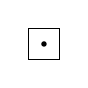
\begin{tikzpicture}%
          \draw (-\dw, -\dw) rectangle (\dw, \dw);
          \fill (0, 0) circle[radius=\dr];
        \end{tikzpicture}%
      }%
      \newcommand{\diceb}%
      {%
        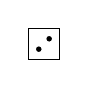
\begin{tikzpicture}%
          \draw (-\dw, -\dw) rectangle (\dw, \dw);
          \fill (-0.33*\dw, -0.33*\dw) circle[radius=\dr];
          \fill ( 0.33*\dw,  0.33*\dw) circle[radius=\dr];
        \end{tikzpicture}%
      }%
      \newcommand{\dicec}%
      {%
        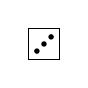
\begin{tikzpicture}%
          \draw (-\dw, -\dw) rectangle (\dw, \dw);
          \fill (-0.45*\dw, -0.45*\dw) circle[radius=\dr];
          \fill (        0,         0) circle[radius=\dr];
          \fill ( 0.45*\dw,  0.45*\dw) circle[radius=\dr];
        \end{tikzpicture}%
      }%
      \newcommand{\diced}%
      {%
        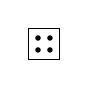
\begin{tikzpicture}%
          \draw (-\dw, -\dw) rectangle (\dw, \dw);
          \fill (-0.38*\dw,  0.38*\dw) circle[radius=\dr];
          \fill ( 0.38*\dw,  0.38*\dw) circle[radius=\dr];
          \fill (-0.38*\dw, -0.38*\dw) circle[radius=\dr];
          \fill ( 0.38*\dw, -0.38*\dw) circle[radius=\dr];
        \end{tikzpicture}%
      }%
      \newcommand{\dicee}%
      {%
        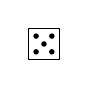
\begin{tikzpicture}%
          \draw (-\dw, -\dw) rectangle (\dw, \dw);
          \fill (-0.5*\dw,  0.5*\dw) circle[radius=\dr];
          \fill ( 0.5*\dw,  0.5*\dw) circle[radius=\dr];
          \fill (       0,        0) circle[radius=\dr];
          \fill (-0.5*\dw, -0.5*\dw) circle[radius=\dr];
          \fill ( 0.5*\dw, -0.5*\dw) circle[radius=\dr];
        \end{tikzpicture}%
      }%
      \newcommand{\dicef}%
      {%
        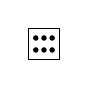
\begin{tikzpicture}%
          \draw (-\dw, -\dw) rectangle (\dw, \dw);
          \fill (-0.52*\dw,  0.38*\dw) circle[radius=\dr];
          \fill (        0,  0.38*\dw) circle[radius=\dr];
          \fill ( 0.52*\dw,  0.38*\dw) circle[radius=\dr];
          \fill (-0.52*\dw, -0.38*\dw) circle[radius=\dr];
          \fill (        0, -0.38*\dw) circle[radius=\dr];
          \fill ( 0.52*\dw, -0.38*\dw) circle[radius=\dr];
        \end{tikzpicture}%
      }%
      \newcommand{\cmapsto}
      {%
        \begin{tikzpicture}%
          \node at (0, 0) {$\mapsto$};
          \clip (-\dw, -\dw) rectangle (\dw, \dw);
        \end{tikzpicture}%
      }%
      \newcommand{\cnum}[1]
      {%
        \hspace*{-0.5em}%
        \begin{tikzpicture}%
          \node[left] at (\dw, 0) {$#1$};
          \clip (-\dw, -\dw) rectangle (\dw, \dw);
        \end{tikzpicture}%
      }%
      \begin{equation*}
        X:\Omega\to\mathbb{R}
        \quad\text{mit}\quad
        \begin{array}{lcr}
          \text{\dicea} & \text{\cmapsto} & \text{\cnum{1}}  \\
          \text{\diceb} & \text{\cmapsto} & \text{\cnum{2}}  \\
          \text{\dicec} & \text{\cmapsto} & \text{\cnum{3}}  \\
          \text{\diced} & \text{\cmapsto} & \text{\cnum{4}}  \\
          \text{\dicee} & \text{\cmapsto} & \text{\cnum{-5}} \\
          \text{\dicef} & \text{\cmapsto} & \text{\cnum{-6}}
        \end{array}
      \end{equation*}
    \endgroup
    Der Erwartungswert dieser Funktion gibt dann
    die durchschnittliche Anzahl von Gummibärchen
    an, um die sich der Vorrat von \xya{} pro
    Runde verändert.
    % </OUTLINE>
  \fi
  \ifoutcome\outcome\par
    % <OUTCOME>
    Für die im Ansatz definierte Zufallsvariable
    $X$ erhält man folgenden Erwartungswert:
    \begin{equation*}
      E(X)=\frac{1}{6}\cdot1
          +\frac{1}{6}\cdot2
          +\frac{1}{6}\cdot3
          +\frac{1}{6}\cdot4
          +\frac{1}{6}\cdot(-5)
          +\frac{1}{6}\cdot(-6)
          =
          %<OCTAVE>
          -\frac{\num{1}}{\num{6}}
          %</OCTAVE>
          %myn2s((1+2+3+4-5-6)/6, 0,0,0,0,1)
    \end{equation*}
    Da der Erwartungswert negativ ist, wird
    \xya{} auf lange Sicht alle Gummibärchen
    an \xxb{} verlieren.
    % </OUTCOME>
  \fi
\end{exercise}
